\documentclass[main.tex]{subfiles}
\begin{document}

\marginpar{Tuesday\\ 2020-12-1, \\ compiled \\ \today}

We defined the neutron-to-proton ratio \(R_{np} = n_n / n_p\), and found 
%
\begin{align}
R_{np} = x_n^3 \qty[\frac{4 (1 + x_n^2)}{x_n^4 + 4 Q x_n^2 / m_n + 4 (Q^2- m_e^2) / m_n^2}]^{3/2}
\,.
\end{align}

In the \(x_n \gg 1\) limit, this is roughly a constant: \(R_{np} \sim 4^{3/2} = 8\).

\begin{figure}[ht]
\centering
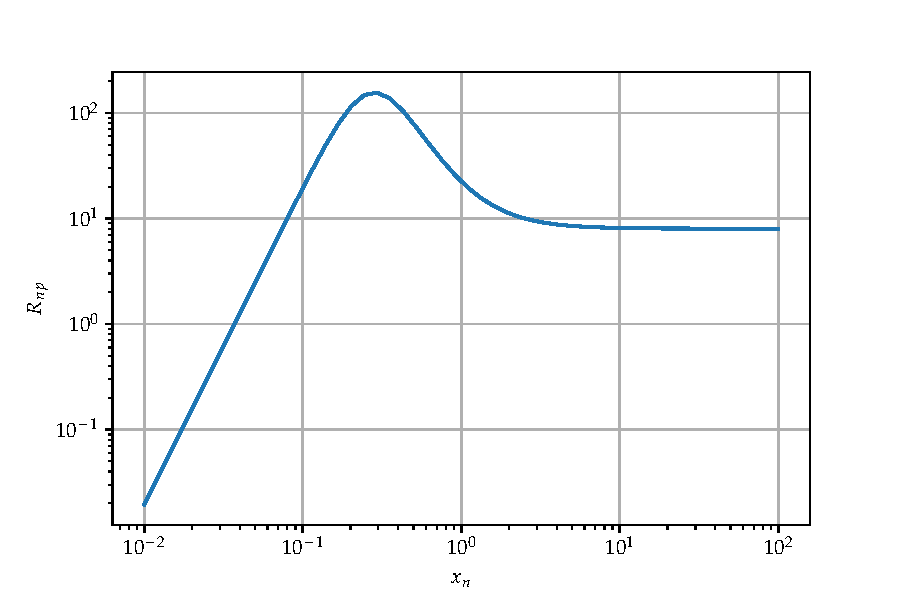
\includegraphics[width=\textwidth]{figures/neutron-proton-ratio}
\caption{Neutron-proton ratio.}
\label{fig:neutron-proton-ratio}
\end{figure}

For heavy nuclei we have the process:
%
\begin{align}
(Z, A) + e^{-} \to (Z-1, A) + \nu 
\,.
\end{align}

Above a certain density we start having neutron ``drip'' from heavy nuclei.

\begin{figure}[ht]
\centering
\includegraphics[width=\textwidth]{figures/NS-interior}
\caption{Stolen image.}
\label{fig:NS-interior}
\end{figure}

\subsection{The URCA and MURCA processes}

At \(T > \SI{e10}{K}\), we will have to account for both photon and neutrino luminosity (\(L_\gamma \) and \(L_\nu \) respectively): 
%
\begin{align}
\dv{E _{\text{th}}}{t} = H - L_\gamma - L_\nu 
\,,
\end{align}
%
where \(H\) is the heating rate. We also know that 
%
\begin{align}
\dv{E _{\text{th}}}{t} = c_V \dv{T }{t}
\,,
\end{align}
%
therefore 
%
\begin{align}
c_V \dv{T }{t} = H - L_\nu - L_\gamma 
\,.
\end{align}

We have the two processes of neutron decay and neutron formation (electron capture). These constitute the direct URCA process. 
URCA was a famous Casino in Rio in the fifties, and the name was proposed by George Gamow, who liked gambling: 
the idea is that if these two processes were to occur at equilibrium then energy would be lost by a NS ``as fast as money is lost at URCA''. This is thus known as a ``fast'' neutrino-producing process.

By momentum conservation, neglecting the momentum of the neutrino,\footnote{It is indeed negligible since this is all happening in a degenerate gas of neutrons, protons and electrons: therefore, their momenta must be very high since the low-momentum states are saturated.} we will have \(\vec{p}_n = \vec{p}_p + \vec{p}_e\); however all three species are degenerate, therefore this equality must also hold for the Fermi momenta. 

By the triangle inequality we know that \(p_{Fn} \leq p_{Fp} + p_{Fe}\), and by charge neutrality we also know that \(n_e = n_p\), therefore  \(p_{Fe} = p_{Fp}\), therefore \(p_{Fn} \leq 2 p_{Fp}\). 

Finally, this yields \(n_n \leq 8 n_p\), or \(R_{np} \geq 8\). Therefore, 
%
\begin{align}
\frac{n_p}{n_n + n_p} \geq \frac{1}{9}
\,.
\end{align}

This contradicts what we found for \(R_{np}\): we learned that. 

We could have exotic particles like hyperons or kaons.
There is no direct evidence for exotica, so first we should look to second order processes, which include a bystander, like
%
\begin{align}
\ce{n} + \ce{n} \to e^{-} + \ce{p} + \overline{\nu} + \ce{n}
\,,
\end{align}
%
which is called the n-channel, or the p-channel, in which the bystander is a proton. 

This is the Modified URCA process, or MURCA. This is slow. 

The neutrinoo emissivity looks like 
%
\begin{align}
\epsilon _\nu^{\text{URCA}} &\approx \num{e27} R(\rho ) \qty(\frac{T}{\SI{e9}{K}})^{6} \SI{}{erg cm^{-3} s^{-1}} \\
\epsilon _\nu^{\text{MURCA}} &\approx \num{e21} R(\rho ) \qty(\frac{T}{\SI{e9}{K}})^{8} \SI{}{erg cm^{-3} s^{-1}}
\,,
\end{align}
%
and the total neutrino luminosity (at constant temperature) is 
%
\begin{align}
L_\nu = \int \epsilon _\nu \dd{V}
\,.
\end{align}

With this, we find that the neutrino luminosity for slow processes (MURCA) is \(L_\nu^{s} = N^{s} T^{8}\), while \(L_\nu^{f} = N^{f} T^{6}\), where \(N^{s}\) and \(N^{f}\) are two constants (with dimensions) whose approximate expressions are given before. 

On the other hand, the photon luminosity can be approximated through blackbody radiation: 
%
\begin{align}
L_\gamma = 4 \pi R^2 \sigma T_e^4
\,,
\end{align}
%
where \(T_e\) is different from \(T\) (typically much lower than it). 
This is due to the presence of an envelope around the neutron star, which emits the bulk of the radiation. 

Typically, we can take \(T = \const\) inside the core, and \(T_e \propto T^{1/2 + \alpha }\), with \(\alpha \ll 1\). 

This then tells us that \(L_\gamma = S T^{2 + 4 \alpha }\). 

We can say that for a degenerate system \(c_V \approx c T\) for some constant \(c\). 

Finally we find 
%
\begin{align}
c T \dv{T}{t} = - L_\nu - L_\gamma 
\,,
\end{align}
%
and as we will see \(L_\nu \gg  L_\gamma \), therefore if MURCA dominates over URCA and photons we have 
%
\begin{align}
cT \dv{T}{t} = - N^{s} T^{8}
\,,
\end{align}
%
which yields 
%
\begin{align}
\frac{ \dd{T}}{T^{7}} &= - \frac{N^{s}}{c} \dd{t}  \\
\frac{1}{6} \qty( \frac{1}{T^{6}} - \frac{1}{T _{\text{in}}^{6}}) &= \frac{N^{s}}{c} (t - t _{\text{in}})
\,.
\end{align}

If \(T _{\text{in}} \gg T\) (which is realistic with SN formation scenarios) we will have 
%
\begin{align}
\frac{c}{6 N^{s}} t^{-1} = T^{6} \implies T \propto t^{-1/6}
\,.
\end{align}

We can make a very similar calculation for the URCA process: this yields  \(T \propto t^{-1/4}\), a steeper decrease. 

The fast process timescale looks like 
%
\begin{align}
\tau^f_\nu = \frac{c}{4 N^{f} T^{4}} = 4 \qty(\frac{c_{30}}{10 N^{s}_{\num{.62}} T^{4}_9}) \SI{}{s}
\,,
\end{align}
%
which is much shorter than the corresponding slow timescale 
%
\begin{align}
\tau^s_\nu = \frac{c}{6 N^{s} T^{6}}  = 6 \qty(\frac{c_{30}}{6 N_{30}^{s} T^{4}_9}) \SI{}{months}
\,.
\end{align}



\end{document}
